
\printMiniToc


\normalInfo{Level design}{Le \anglicisme{level design} est l'art de créer des niveaux bien équilibrés, fun à jouer et variés. C'est l'art de bien disposer les obstacles, récompenses et bâtiments pour que la difficulté soit adaptée. La carte doit présenter suffisamment de challenges pour motiver les joueurs, sans être excessivement difficile ce qui les empêcherait d'avoir une bonne expérience du jeu.}

\warningInfo{Niveaux déjà préparés}{Seul le premier acte du jeu est défini de manière détaillée. Le reste du jeu est brièvement décrit à la fin de ce chapitre.}

\section{Premier acte}
\label{sec:premierActe}

\subsection[Niveau 1 --- Course-poursuite avec la garde]{Premier niveau --- Course-poursuite avec la garde}
\label{sec:coursepoursuiteGarde}
\warningInfo{Un niveau d'importance}{Le premier niveau est crucial, c'est à la fois la scène d'exposition, l'opportunité de découvrir l'univers du jeu et l'apprentissage nécessaire des contrôles. S'il est bien réussi et fluide, le joueur pourra prendre plaisir à jouer et s'attacher à son personnage.}

Dans le premier niveau d'\nomJeu\ qui se déroule dans Redel, le joueur incarne Kida, l'héroïne. Elle est accompagnée par Lenaï, sa grande s\oe ur. Les premiers instants servent à l'apprentissage des commandes: se déplacer, courir, s'accroupir, sauter, etc. C'est la prise en main.

Puis vient l'élément déclencheur: deux gardes qui passent par l'avenue marchande, oublient négligemment un petit coffre au bord de l'étalage où ils viennent d'acheter de quoi manger. Kida ne peut s'empêcher de s'approcher pour observer la boîte mystérieuse. Tentée, elle la saisit sans avoir vraiment l'intention de la rendre. Mais au moment de commettre son délit, les gardes, ayant noté leur inadvertance, se retournent. À la vue des deux s\oe urs, ils leur hurlent d'arrêter; ces dernières prennent leurs jambes à leur cou et une course-poursuite s'engage.

Pour réussir le niveau, le joueur doit passer à temps les obstacles qui lui sont présentés afin de pouvoir s'enfuir. Ces empêchements ne doivent présenter qu'une faible difficulté pour permettre au joueur à la fois de s'habituer aux commandes et d'avoir une première impression aussi bonne que possible du jeu.

À la fin du niveau, Kida réussit à s'enfuir avec le coffre mais Lenaï est capturée et emmenée par la garde. Cet élément sera la cause des multiples péripéties qui s'ensuivront.

\normalInfo{Niveau de type \anglicisme{alley}}{Ce niveau est dit de type \anglicisme{alley}: à savoir, le joueur n'est pas libre de se balader selon sa propre volonté. À l'inverse, pour réussir le niveau, il doit suivre avec succès un chemin prédéfini.}

\subsection[Niveau 2 --- À la recherche de Lenaï]{Deuxième niveau --- À la recherche de Lenaï}
\label{sec:rechercheLenai}
\warningInfo{Objets à débloquer dans ce niveau}{\begin{itemize}
		\item Bâton de bois
		\item Trois sorts majeurs
		\item Tyrolienne
		\item Sarbacane
		\item Une recette de poison
	\end{itemize}
Si le nombre d'objets à débloquer est aussi important dans ce niveau, c'est que cela permet de lancer immédiatement le joueur au c\oe ur de l'action; dès le début du jeu, il possède des moyens pour interagir avec le monde virtuel qui l'entoure.
}

Le deuxième niveau débute le jour suivant. Kida part à la recherche de sa s\oe ur. Cette quête va cependant être entravée par le fait que la garde a bouclé les sorties du quartier pour retrouver le coffre volé; tout le monde est fouillé. Ainsi, l'héroïne se retrouve bloquée dans Redel. Faute de mieux, elle cherche à ouvrir le coffre volé, qui semble avoir nettement plus de valeur que ce qui aurait pu être supposé dans un premier temps.

La première tâche du joueur sera d'ouvrir le coffre. Il devra pour cela s'introduire par les toits dans la boutique du serrurier absent et utiliser ses machines pour créer une clé adaptée (puzzle\definition). Lorsque le coffre s'ouvre, un étrange animal en bondit. C'est la première rencontre avec un esprit de la Nature: Tia, l'écureuil vif et sauvage. La créature dit à Kida d'aller voir Maïnin, le vieux sage, puis s'enfuit en courant.

Le vieil homme, qui est en fait le gardien de l'accès au sanctuaire, y introduit la jeune fille (puzzle\definition\ pour activer le passage). Kida y rencontre Tia, qui lui explique les bases du fonctionnement de l'énergie verte, lui confie les trois premiers totems et le bâton de bois (voir les sections sur le \nameref{chap:gameplay}). L'esprit lui parle également d'un passage secret au c\oe ur du quartier naturel. Il donne accès à la rivière, puis à la tour de Gaamon dans laquelle Lenaï est sûrement enfermée.

Pour accéder à ce nouveau quartier, il faut résoudre toute une série de quêtes et de sous-quêtes pour finalement débloquer le passage indiqué par un \enquote{?} sur la maison mitoyenne de celle du cordonnier.

Au court du début de ce niveau, le joueur doit tirer profit des chemins sur les toits pour accéder aux endroits difficiles, pénétrer dans les maisons fermées et avancer dans l'histoire. Une carte des toits de Redel est donnée à la figure \ref{fig:carteQuartierPauvre}. Cet élément du Gameplay ajoute une dimension supplémentaire au jeu; le joueur doit utiliser le \enquote{z-axis} (que l'on pourrait traduire en français par la dimension verticale). Les passages par les toits ajoutent de plus un côté fun au jeu de même que les tyroliennes sur les rues, les passages secrets et les récompenses à débloquer par le joueur. Ils permettent de diversifier la façon de jouer.

Une fois le passage ouvert, un nouveau lieu est débloqué: le quartier naturel caché de Redel. Le joueur se voit alors confier par les Naturels une sarbacane, quelques dards et une première recette de poison. Si le joueur a déjà collectionné suffisamment d'ingrédients, il peut confectionner des dards supplémentaires. Les habitants du quartier ouvrent ensuite le passage situé sous la statue de Gaamon, au milieu de la place. L'héroïne peut ainsi accéder à la rivière et par extension, à la Tour.

\normalInfo{Niveau de type \anglicisme{island}}{Ce niveau, à l'inverse du précédent, représente un niveau de type \anglicisme{island}. Cela signifie que le joueur est libre de ses mouvements et peut aller où bon lui semble. Un autre terme pour décrire ce type de niveau serait semi open-world\definition.}

\begin{figure}[ph!]
	\centering	
	\subfloat[Plan du quartier pauvre]{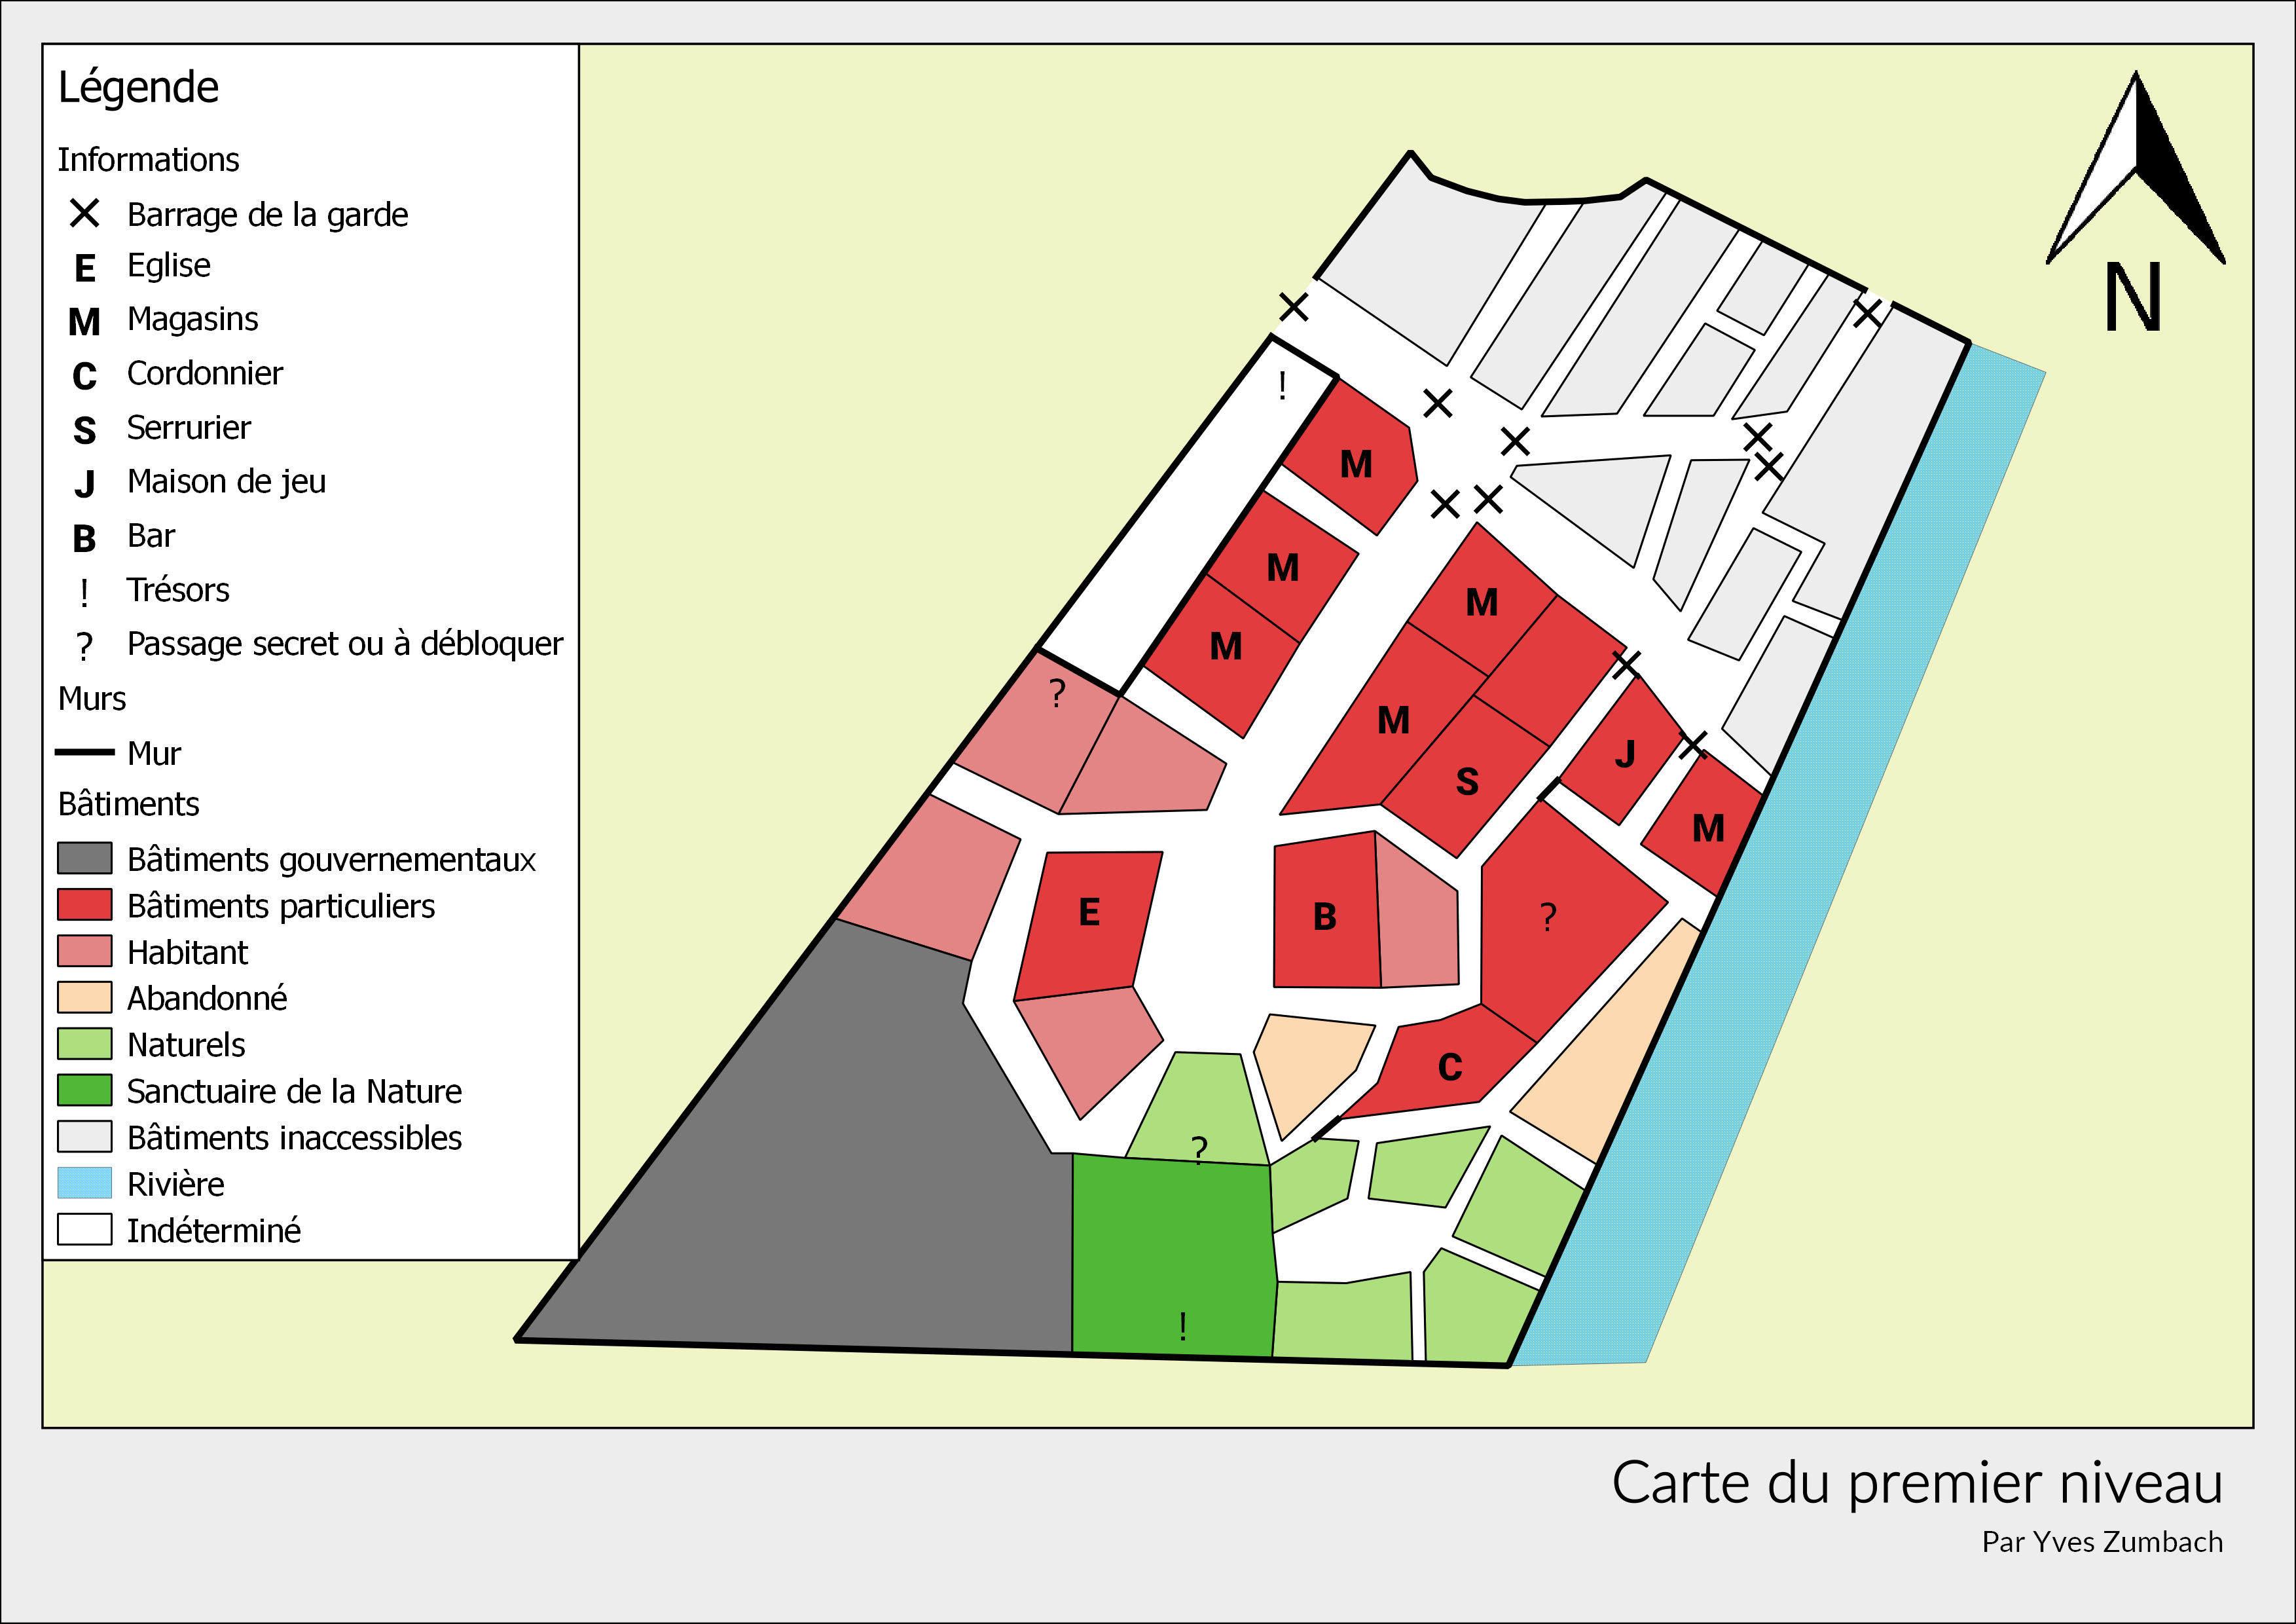
\includegraphics[width=\textwidth]{images/LevelDesign/cartePremierNiveauIndicationsGameplay.png}}
	
	\subfloat[Plan des toits]{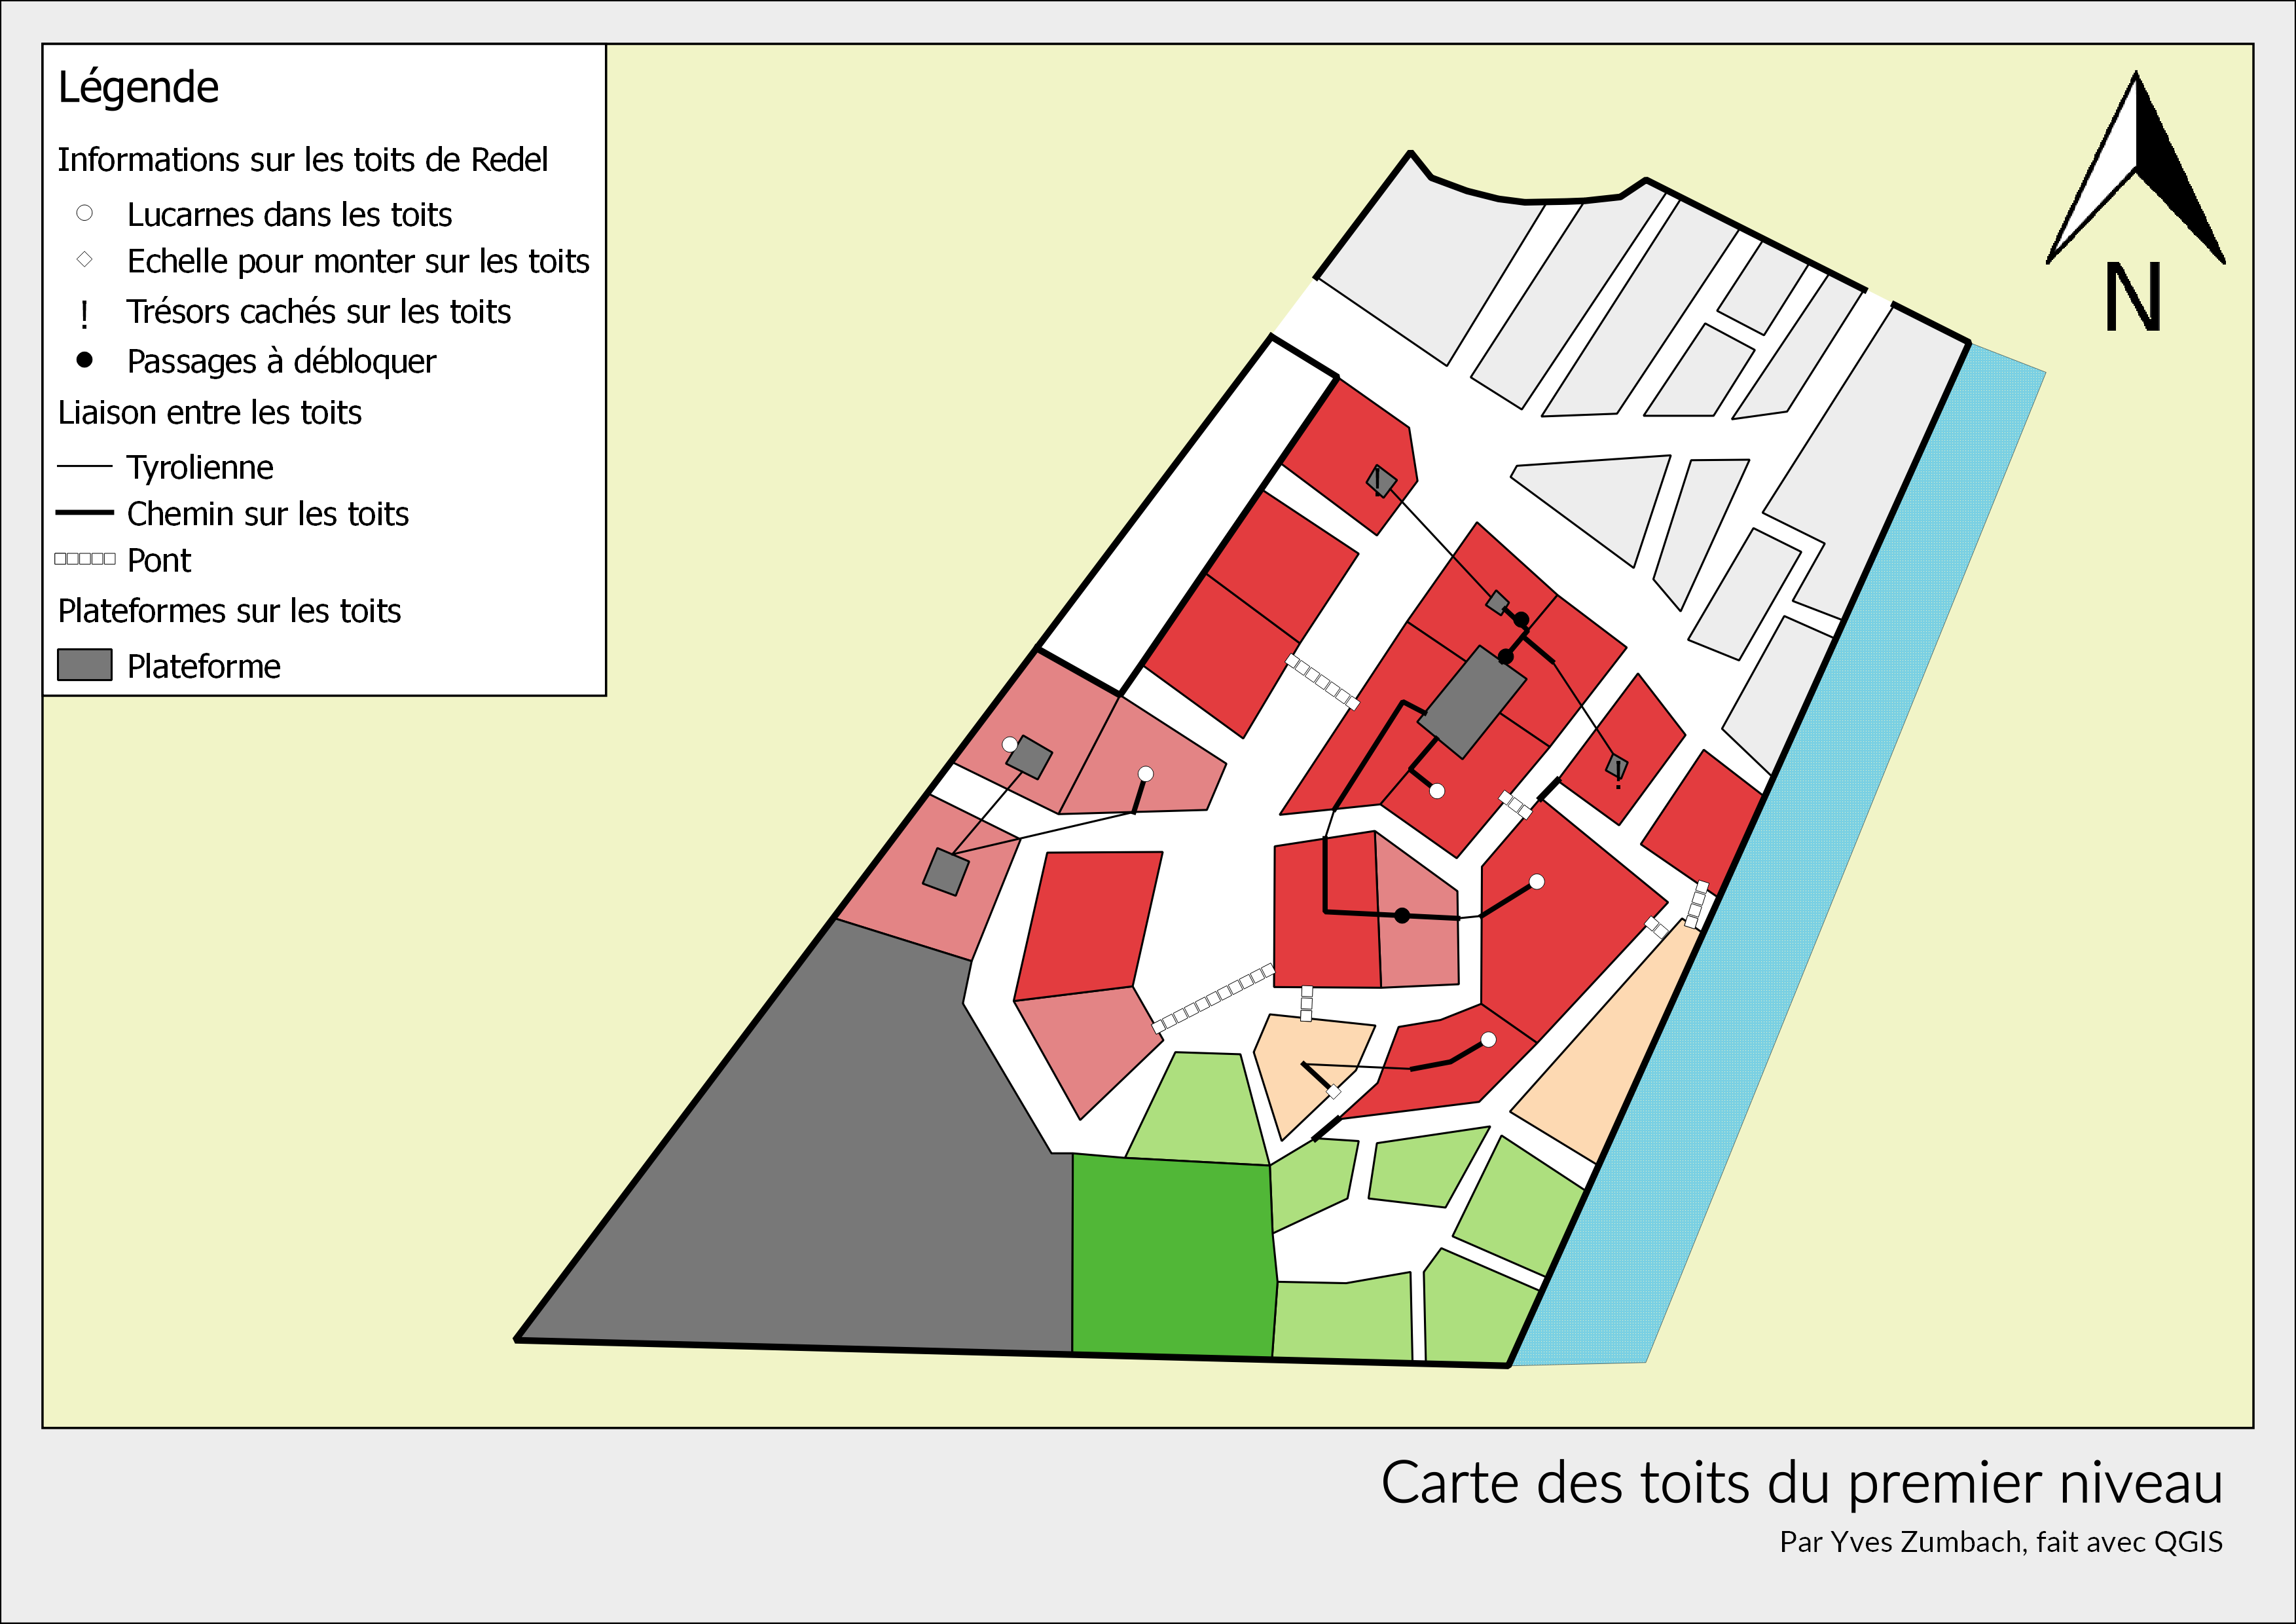
\includegraphics[width=\textwidth]{images/LevelDesign/carteToitsPremierNiveau.png}}
	
	\caption{\label{fig:carteQuartierPauvre}Cartes de Redel (réalisé à l'aide du programme Quantum GIS)}
\end{figure}


\subsection[Niveau 3 --- Dans l'antre du démon]{Troisième niveau --- Dans l'antre du démon}
\label{sec:entreDemon}
Kida pénètre dans le château de Gaamon par les souterrains. Ce niveau est un temple\definition. Il s'agira de trouver les cachots où Lenaï pourrait être enfermée. Le joueur le fera en résolvant des puzzles\definition\ pour accéder aux pièces suivantes (portes bloquées ou fermées) et éviter les ennemis (se référer à la partie \enquote{\nameref{chap:gameplay}} pour plus de détails).

Les objectifs intermédiaires du niveau seront de trouver la carte de la Tour, collecter des objets et des clés afin de pouvoir ouvrir les portes vers les salles suivantes.

Finalement, en arrivant aux cachots, Kida ne trouvera que des cellules vides... Aucune trace de Lenaï. C'est à ce moment que le boss\definition\ apparaît sous la forme d'une grande femme en armure. Le combat s'engage immédiatement. Kida se défend du mieux qu'elle peut, mais elle ne peut résister face à son adversaire parfaitement équipé pour le combat, aux armes aiguisées et techniques évoluées. Le joueur devra cependant survivre un certain temps au combat pour pouvoir avancer dans l'histoire. Il finit par se faire renverser et atterrit durement sur le sol, désarmé (cet élément pourrait être narré avec une cinématique). L'antagoniste lève son arme afin de porter le coup de grâce. Mais l'espace d'un instant, un éclair de doute traverse les yeux de la guerrière. Au même instant, Kida reconnait sa grande s\oe ur sous le masque terrifiant qu'elle porte: c'est contre Lenaï qu'elle s'est battue! L'hésitation à porter le coup fatal suffit à Kida qui profite de l'ouverture pour s'échapper, se précipiter vers la fenêtre la plus proche et sauter droit dans les douves... à l'extérieur de la ville.

\criticalInfoDarkRed{Importance du troisième niveau}{Le troisième niveau est véritablement la clé de voûte de l'histoire. On y découvre que Lenaï est passée du côté de Gaamon. Cet élément capital sera la cause des multiples péripéties de l'histoire d'\nomJeu.

Ce retournement étrange s'explique par le fait que Gaamon, le père de Lenaï, accueille, à son arrivée dans la Tour, sa fille disparue comme jamais la jeune femme n'avait été traitée. Il demande à la garde de la libérer de ses liens et l'emmène au c\oe ur de la Tour. Là, il se comporte comme le père qui a toujours manqué à Lenaï. Il lui apporte l'attention, l'affection et l'amour dont elle avait toujours rêvé, et qui lui faisait cruellement défaut depuis la mort de leur mère. Lenaï se réfugie dans ce havre de paix et de bonheur que son père crée autour d'elle. C'est pour défendre cette relation, qu'elle accepte de commettre certains actes parmi les plus répréhensibles. Son père l'aime et la protège mais, implicitement, elle sait que pour conserver son amour, il lui faut accepter de devenir celle que Gaamon veut qu'elle soit: son bras armé, la générale de ses troupes. Le revirement est donc brutal et Lenaï commet de nombreux crimes afin de conserver sa situation.
}

\section{Jouer Lenaï}
La plupart des niveaux sont joués avec Kida. Cependant, certains utiliseront Lenaï comme personnage. Cela apporte un énorme avantage technique: la réutilisation des niveaux et contenus déjà réalisés. En même temps, cette façon de faire offre des points de vue diversifiés à l'histoire, ce qui la rend plus intéressante. Mieux encore, cela permet au joueur d'avoir un aperçu de la vie de Lenaï. C'est ce dernier point qui a le plus de valeur pour moi. Il permet d'approfondir le personnage de Lenaï, de Gaamon et le gameplay: lorsqu'on joue Lenaï, on est forcé d'exécuter les ordres de Gaamon, il faut donc compléter les missions données par le grand ennemi du jeu.

C'est premièrement une façon de découvrir Gaamon, ainsi que sa base. Cela permet au joueur d'obtenir un aperçu des forces ennemies, et de fonctionner comme un espion dans l'antre ennemi. Ces niveaux seront aussi l'occasion d'explorer la relation entre Lenaï et Gaamon, à la fois paternelle et ambivalente car Lenaï, bien qu'elle soit \enquote{ensorcelée}, perçoit bien que ce qu'elle fait est immoral et injuste.

Enfin, le tyran commandant à ses subordonnés des missions à l'éthique hautement critiquable comme collecter des impôts énormes chez les paysans autour de la ville, aller éradiquer la Nature sur une surface toujours grandissante autour de la cité, etc, ces missions seront l'occasion de proposer un choix au joueur quant à leur résolution. Par exemple pour la collecte des impôts, le joueur pourra mettre à sac les maisons des habitants incapables de payer pour trouver jusqu'à la dernière pièce, une solution simple et efficace, ou alors faire l'effort de  trouver lui-même des pièces (la possibilité lui en sera donné) pour aider les personnes les plus en difficulté.



\section{Deuxième acte}
\label{sec:deuxiemeActe}
Kida se retrouve hors des murs pour la première fois de sa vie. Elle doit s'habituer à un nouveau mode de vie plus rural, plus sauvage et découvrir les populations environnant \nomVille. Ces personnes sont pour la plupart des renégats ou des paysans ayant fui lors de la création de la ville. La vie est très dure. Gaamon, s'il tolère ces personnes, ne les épargne pas pour autant. Elles se font voler par la garde, les impôts prélevés sont ridiculement élevés, parfois même, Gaamon envoie ses machines détruire une ou deux maisons afin de tester leur efficacité. Ces gens ont donc appris à se cacher et savent détecter l'arrivée des soldats. Beaucoup parmi eux seraient même près à se battre mais la supériorité militaire de Gaamon est indubitablement écrasante. Ils se tiennent prêts au combat mais attendent l'occasion opportune et survivent en attendant.

Kida y apprend la légende fantastique du peuple des \nomNaturels s, un peuple technologiquement extrêmement avancé, beau, raffiné et puissant. C'est ce mythe qui fait espérer encore les exclus; pour eux, il existe encore une chance. C'est ce mythe aussi qui va décider Kida. Pour sauver sa s\oe ur, elle se met à la recherche de ce peuple fantastique, convaincue que si elle arrive à bâtir un monde meilleur avec l'aide de ces gens, son aînée verra l'absurdité de ses actions et qu'elle la rejoindra.

Piste après piste, bribe après bribe d'information, son chemin la conduira finalement à découvrir, caché au fond d'une forêt sombre et majestueuse, un très ancien temple à l'architecture gracieusement étrange, sortie tout droit d'un autre âge: un temple teluran. C'est en haut de ce dernier qu'elle trouve un engin volant qui, une fois réveillé, la conduit automatiquement sur les hauts-plateaux, où le peuple persécuté a trouvé refuge. Kida vient de trouver un des derniers moyens de retrouver les Telurans que ces personnes éclairées avaient laissé aux Hommes.

\section{Troisième acte}
\label{sec:troisiemeActe}
Une fois arrivée chez les Telurans, Kida découvre que le peuple magnifique en lequel elle espérait n'est plus que l'ombre de lui-même. Les persécutions incessantes de Gaamon ont fini d'achever les dernières merveilles de ce peuple: le palais royal tombe en ruine, l'art qui en faisait jadis la gloire est maintenant tombé en ruine, oublié, mais surtout, les secrets de l'énergie verte sont tous perdus. La vie est devenue dure. Sans sa source vitale, la glorieuse nation survit à peine; tous les habitants travaillent aux champs ou dans les ateliers et la connaissance, la science, la notion de beau, d'élégant, l'essence même du peuple se perdent inexorablement.

Profondément choquée par cet état pitoyable, que les Telurans ne peuvent rien pour sa s\oe ur, Kida part à la recherche des secrets de l'énergie verte. Après de longues recherches, elle rencontre finalement l'esprit de la Nature Léo dans la forêt de Tylor. Les esprits ne prennent normalement pas part aux affaires du monde et se contentent d'être spectateur des époques et des peuples naissants, arrivant à leur apogée puis déclinants. Cependant, confronté au récit qui lui est fait, Léo, esprit impulsif, décide d'enseigner à Kida les secrets de la grande salle.

Cette connaissance retrouvée et la grande salle remise en marche, la cité telurane retrouve d'elle-même sa gloire passée, les bâtiments renaissent, les animaux reviennent parmi le peuple, l'art et la musique redeviennent ce qu'ils auraient toujours dû être et s'élèvent d'eux-mêmes, la beauté de la vie se mêle à nouveau au chant de la Nature.

\section{Quatrième acte}
\label{sec:quatriemeActe}
À ce point du jeu, le joueur a déjà joué plusieurs niveaux dans la peau de Lenaï. Un ultime niveau de ce type permet de mettre en évidence l'impact que les horreurs de Gaamon ont sur Lenaï. Elles la poussent à se révolter contre l'image paternelle et elle fuit la cité humaine à bord d'un dirigeable blindé vers les hauts-plateaux où elle retrouve les Telurans et Kida. Cette dernière apprend ainsi l'identité de son géniteur, elle n'est autre que la fille de son pire ennemi. Et si tout le monde se montre méfiant d'abord à l'égard de Lenaï, les informations alarmantes qu'elle apporte dissipent rapidement les soupçons: Gaamon a atteint la phase finale de son plan; il a prévu la destruction totale de toute Nature... et des Telurans. 

Il a constitué une immense armée de machines, amassées devant les murailles de Murtos, qu'il s'apprête à lancer sur toutes les forêts d'Éluria. Kida, aidée de sa s\oe ur, doit donc retrouver les derniers secrets manquants de l'énergie verte afin de donner aux Telurans suffisamment de puissance pour affronter et démanteler les troupes mécaniques. Et ce sont les mystères des machines volantes teluranes qu'il faut retrouver pour accomplir un tel miracle.

On peut ensuite imaginer un immense combat aérien entre les machines volantes et légères des Telurans et les dirigeables blindés des factions humaines. Les humains prenant l'avantage, Kida comprend que le seul moyen de remporter la victoire est de tuer son père. Kida et Lenaï, côte-à-côte à bord d'un aéronef propulsé à l'énergie verte, se jettent alors sur la tour de verre depuis laquelle leur père contrôle ses forces. Le combat final entre Gaamon, utilisant toutes ses machines, et les deux s\oe urs dévoile le dernier secret du monstre: il a remplacé la plupart des parties de son corps par des membres robotisés. Finalement le tyran est défait. Son armée tombe alors immédiatement en pièce: Gaamon était la clé qui maintenait l'univers des Hommes debout.

Kida et Lenaï pénètrent dans le c\oe ur sacro-saint de la Tour, la seule pièce que Gaamon avait toujours interdite à Lenaï. Elles y découvrent une salle aux couleurs chatoyantes; un magnifique portrait de Miya est accroché glorieusement au milieu du mur faisant face à la porte d'entrée. Sous ce dernier sont couchées de fraîches et belles fleurs orange. L'histoire se termine avec la découverte d'un vieux livre, sous les fleurs, narrant le conte tant affectionné de Miya et Gaamon dont ils ont tiré le nom de leur première fille Lenaï.

